\chapter{Distributed Sensor Networks for Air Quality Assessment}\label{ch:air-network}

\section{Measurement of Particulate Matter}

\subsection{Measurement Methods}

Describe federal method (gravimetric analysis) and optical particle counter
designs based on Mie theory.

\subsection{Problems of Scale}

Describe why we need dense sensor networks, specifically to address the relevant
spatio-temporal scales that are missed by averaging to suggested EPA standards.

Cite Prabuddha's paper and discuss value of dense sensor networks for providing
in-situ reference data which can be used to calibrate remote sensing data
products - highlight the application of PACE e.g. for black-carbon.


% \section{Low Cost Sensors for Real-Time PM Monitoring}

% \subsection{Sensor Design}

% include discussion of limitations, e.g. known problem of hygroscopic growth,
% which is why we incorporate a battery of sensors including sensors for
% meteorological parameters which can be used to post-process PM data for humidity correction.

% \subsection{Sensor Networking}


\section{A Low Cost Sensor Network For Air Quality Monitoring}

The highly expensive cost to acquire, calibrate, and maintain reference grade air quality monitors makes it challenging to assess the importance of spatial and temporal variability on local air quality. Since factors such as weather, terrain, traffic, and the distribution of other sources can all effect local air quality, the development of low-cost sensing solutions is vital to address risks of poor air quality on local communities. To address this gap, we have developed a hierarchy of low-cost air quality monitors which we have deployed throughout the Dallas Fort-Worth (DFW) metroplex. In this section, we describe the relevant sensor types as well as a robust data processing and visualization pipeline developed to enable open access to high quality data.

The sensor network is comprised of a combination of two types of nodes: \textit{Central Nodes} and \textit{LoRa Nodes}. The central nodes are designed to be deployed in locations with where dedicated power is available. Each contains a variety of sensors including Particulate Matter, VOCs, $\mathrm{CO_2}$, $\mathrm{NO_X}$, ionizing radiation, incident light intensity, sound levels, as well as meteorological variables including temperature, pressure, relative humidity, and dew point. The powered Central Nodes are equipped with a cellular modem to facilitate data transfer from the field.

Each Central Node supports a collection of ~10 LoRa nodes (named for the LoRa long rage wireless transmission protocol) which can be separated by distances up to ~5 km or more if line of sight is established. These smaller sensors are self powered using a combination of battery and solar cells, and each measures a similar array of relevant air quality metrics including particulate matter concentrations, gas concentrations, and meteorological parameters. Designs for the two node types are illustrated in Figure \ref{fig:mints-nodes}.
\begin{figure}[!hbt]
  \begin{subfigure}{.5\textwidth}
    \centering
    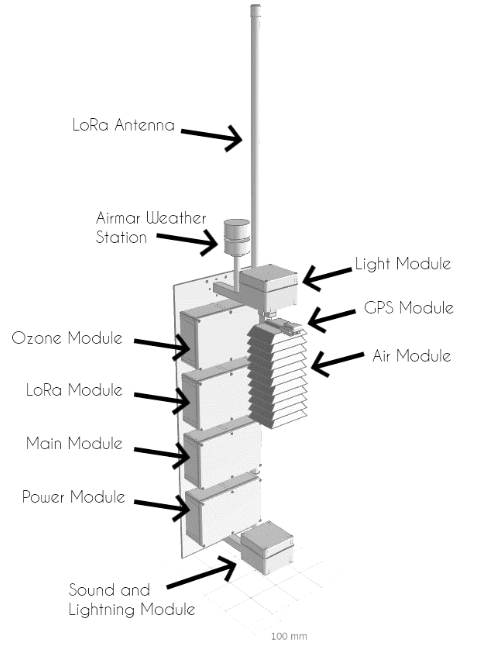
\includegraphics[width=.8\linewidth]{air-network/central-node.png}
    \caption{A 3d model of a Central Node}
  \end{subfigure}
  \begin{subfigure}{.5\textwidth}
    \centering
    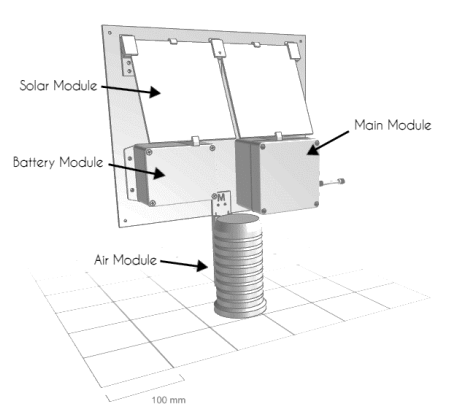
\includegraphics[width=.8\linewidth]{air-network/lora-node.png}
    \caption{A 3d model of a LoRa Node}
  \end{subfigure}
  \caption{Two types of nodes from the MINTS Air Quality network.}
  \label{fig:mints-nodes}
\end{figure}

Using the LoRaWAN protocol, the Central and LoRa nodes form a low power, wide area network by which data packets from each LoRa node are transmitted in real time to the nearest Central Node. Using their inbuilt cellular connection, the central nodes are then able to pass sampled data to a data processing backend using an MQTT publish-subscribe model. As the primary goal of this network is to provide detailed, real-time air quality data, we have developed a public facing website, \url{http://SharedAirDFW.com}, to visualize the current and historic measurement at each sensor location together with 6-hour wind forecasts from NOAA and weather radar. Figure \ref{fig:sharedair-site} shows a sample screenshot of the site.
\begin{figure}[!hbt]
  \centering
  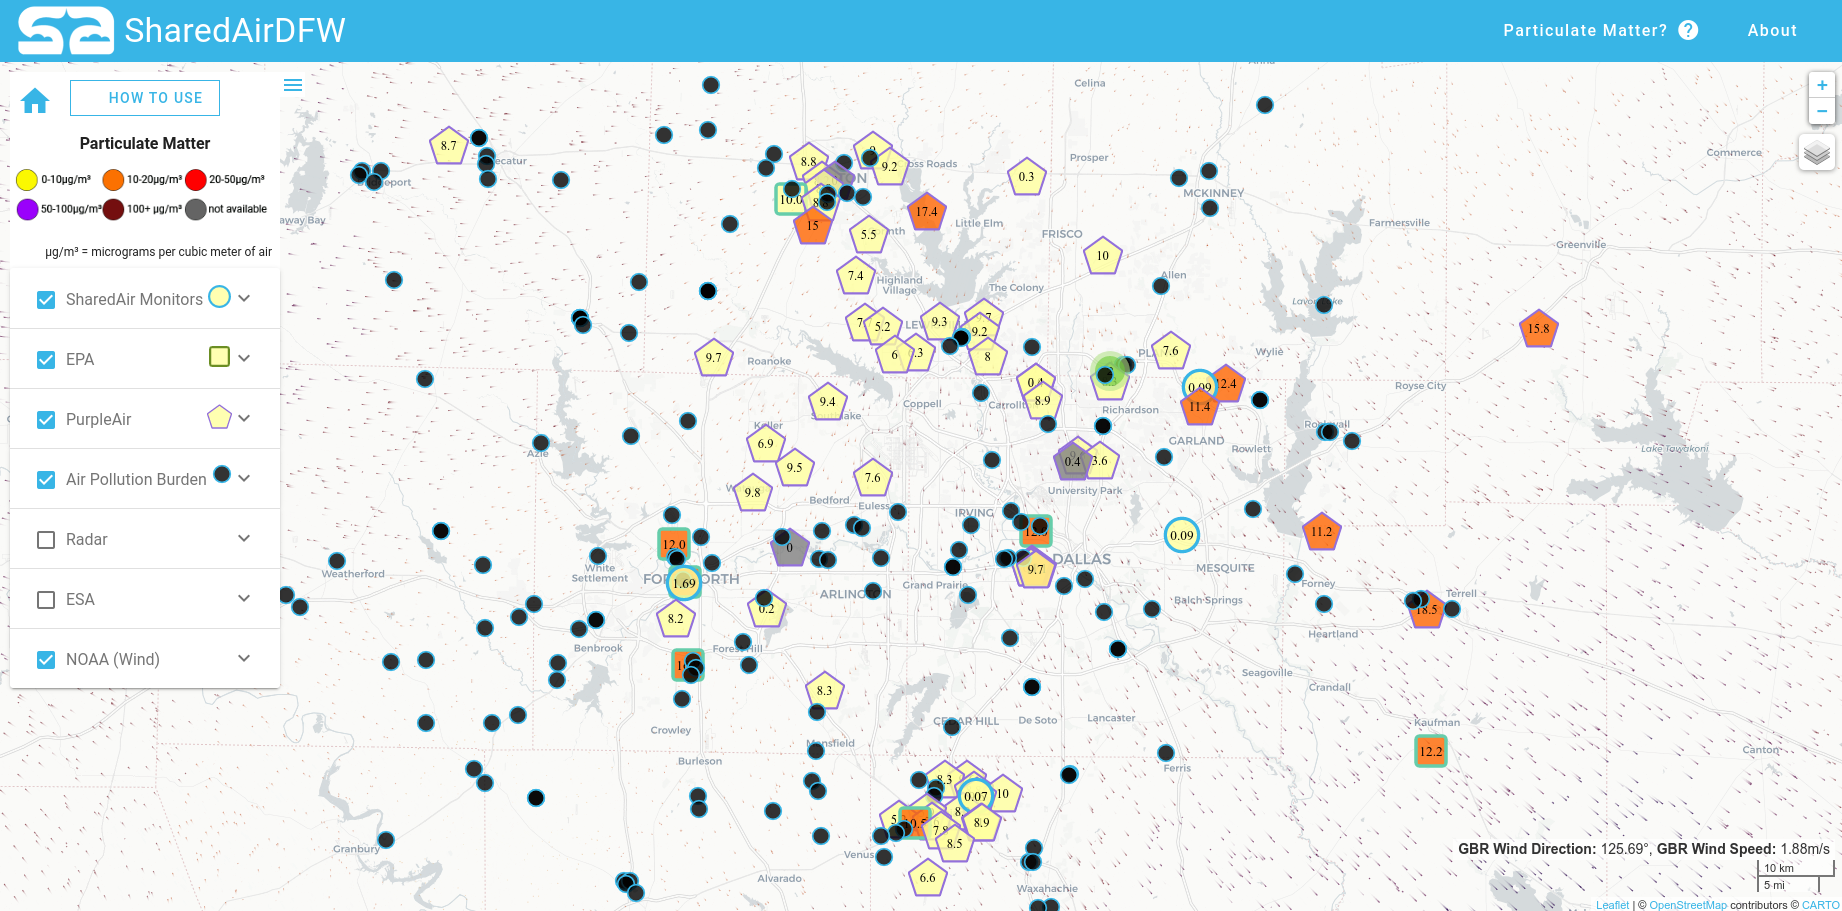
\includegraphics[width=0.85\columnwidth]{air-network/sharedairdfw-homepage.png}
  \caption{The interactive SharedAirDFW website show casing real time data streams from the MINTS sensor network.}
  \label{fig:sharedair-site}
\end{figure}




\section{Towards Real-Time Assessment and Data-Driven Decisions}


\subsection{The Data Pipeline}

Describe docker and containerization. Goal: simple, maintainable framework which
can easily scale as additional sensors are incorporated.

The entire pipeline should be easily reproducible to enable local development
and make it straight forward to transition to cloud-based computing via Amazon
EC2 and other cloud services.


In order to automate data collection, processing, analysis, and long-term storage, a containerized pipeline was developed as illustrated in Figure \ref{fig:dashboards}.
\begin{figure}[!hbt]
  \begin{subfigure}{.2\textwidth}
    \centering
    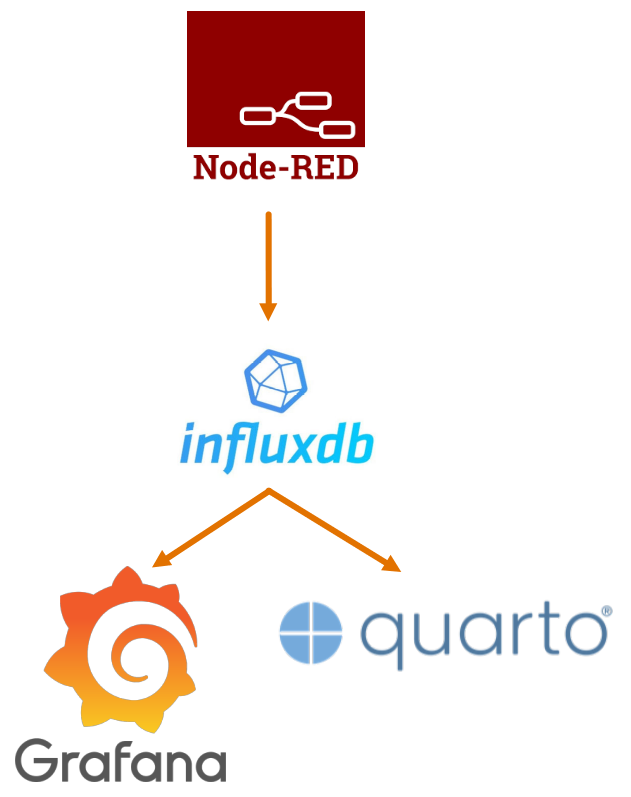
\includegraphics[width=0.85\columnwidth]{air-network/docker-elements.png}
    \caption{}
  \end{subfigure}
  \begin{subfigure}{.8\textwidth}
    \centering
    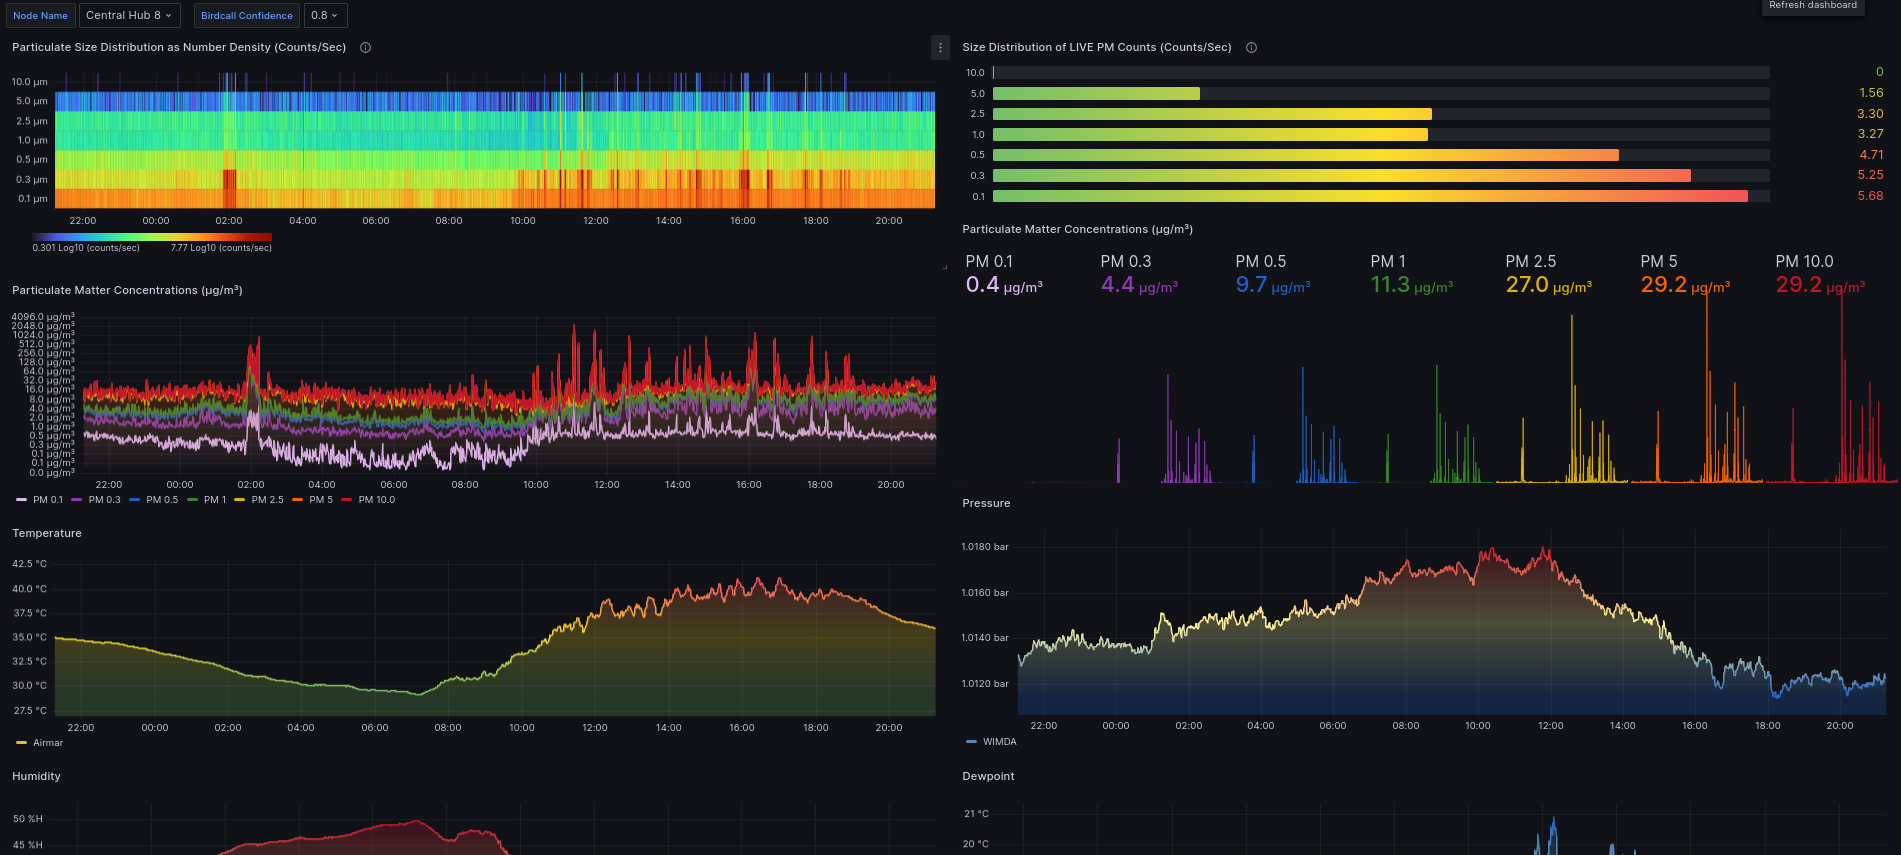
\includegraphics[width=.8\linewidth]{air-network/grafana-dashboard-1.png}
    \caption{}
  \end{subfigure}
  \caption{The backend infrastructure developed to support the MINTS sensor network.}
  \label{fig:dashboards}
\end{figure}
This pipeline is composed of 5 tools that utilize containerization for reliable development and deployment.
\begin{itemize}
\item \textbf{NodeRed}: This tool developed by IBM allows the creation of complex data processing pipelines by defining directed acyclic graphs (DAGs) composed of individual processing nodes. We utlize this tool to subscribe to each sensor's relevant MQTT topic and decode the data packets into the relevant sensor measurements. At the end of each sensor pipeline, the data are then injected into the InfluxDB time series database. A key advantage of NodeRed is that the wide array of pre-existing nodes enables a no-code solution that is easy to maintain.
\item \textbf{InfluxDB}: This is a open source time series database optimized for large cardinality datasets. By storing processed data in InfluxDB, we are able to provide easy queryable access to real time and historic data.
\item \textbf{Grafana}: This tool is an open source visualization platform for creating interactive dashboards. We utilize Grafana to create detailed, real-time displays for each sensor in the network that we can use to observe \textit{all} incoming measurements as well as identify pollution events and monitor sensor status.
\item \textbf{Quarto}: This tool allows the generation of automated analysis reports by using a literate programming paradigm built on top of Jupyter Notebooks. By using quarto we are able to automatically perform daily, weekly, monthly, and annual analyses for each sensor in the network and collect the results into formatted PDFs or a static website. We are developing analysis using quarto together with Julia, Python, and R to facilitate detailed report generation and provide actionable insights.
\item \textbf{Open Storage Network}: With help from Dr. Chris Simmons, we have developed a pipeline for long term data storage utilizing the Open Storage Network to provide open access to historic sensor data stored in the popular S3 format.
\end{itemize}
Individual sensor dashboards are made publicly available at \url{http://mdash.circ.utdallas.edu:3000}. Historic data are updated daily at \url{https://portal.osn.xsede.org/s3browser//?bucket_path=https://ncsa.osn.xsede.org/ees230012-bucket01}.



%\subsection{Live Dashboards}


\subsection{Automated Reports}

Highlight reproducibility as a key analysis criterion






